\chapter{Introduction and State of the Art}
\label{c-intro}

\section{Neuroscience, neurons and their dynamics}
% \textit{What are neurons, its dynamics and what are the To-Dos}
Neuroscience is a wide and challenging field in science. It faces crucial questions in science, such as what are the neural mechanisms in the brain activity, how can those mechanisms outcome as human cognition or behavior, how is the information processed and transferred through neural activity, how are neural disease generated and how can we detect and treat them. 
These questions and many more have been open problems that have intrigued scientific community since the first steps on the field. Neuroscience was born as a discipline from physiology, biochemistry and anatomy, that agglutinates all these questions and more. As a broad field, it is approached from distinct perspectives. Thus, it is usually referred to by its subfields, e.g. Neurobiology, Neurophotonics, Neuropharmacology, Clinical Neuroscience, Developmental Neuroscience, Systems Neuroscience, Cognitive Neuroscience, Computational Neuroscience. All these fields aim to explain the brain performance either as a whole or part of it, lead by different techniques and approaches which have even generate new fields, such as Neuroimaging.

We cannot think or discuss about neuroscience without highlighting the work by Santiago Ramón y Cajal, crucial in the firsts steps on the understanding of brain dynamics \parencite{de_carlos_historical_2007,de_castro_editorial_2016,delgado-garcia_cajal_2015,de_castro_cajal_2019}. The idea of the "neuron doctrine" was a boost on the study of the brain, explaining and describing the structure of individual cells called \textit{neurons} that are able to connect and thus communicate by \textit{synapses}. In Figure \ref{cajal-neuron} there is one of his famous drawings of the description of a neuron.

\begin{figure}[htb!]
    \centering
    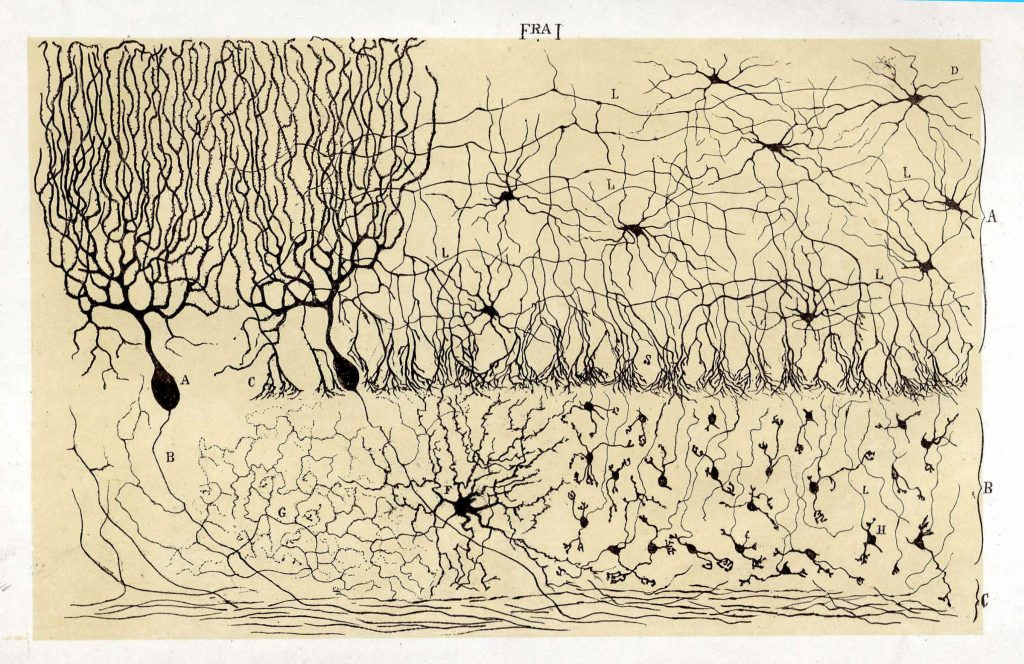
\includegraphics[width=\textwidth]{img/intro/CajalCerebellum.jpeg}
    % https://es.wikipedia.org/wiki/Doctrina_de_la_neurona#/media/Archivo:CajalCerebellum.jpg
    % https://microbioblog.es/la-fascinante-historia-de-la-reazione-nera
    \caption{Representation of Cerebellum neurons by Ramon y Cajal}
    \label{cajal-neuron}
\end{figure}

From that starting point there have been important findings in the neurons types and structures, such as Glia cells \ref{}. 

Although as we have seen brain is a complex system and we could study it from many different prisms, in this thesis we follow a bottom-up approach. So we will analyze experimentally and theoretically the neural activity at ionic channels and small circuits (few synapses). Moreover, it follows a Neurocomputational perspective, that will be developed in detail in subsection \label{computational neuroscience}. In the following lines I will describe the basis of neural activation from a computational perspective, focusing not in their molecular properties but in the change of voltage that they are able to produce and how that inter-operates. 

\subsection{Neural activation}
Neurons are cells composed by axons (the information transfer tube), dendrites (the information reception point) and synapses (the process of information transfer). Also, as any other cell has a soma, where activity is processed. \todo{revisar}
We can find two big types of synapses, electrical or chemical, depending on how is the process of information transferring. In figure \ref{synapse-types} there is a representation of both kinds. The main difference between them relay on how does the communication occur. Chemical synapses occur through the mediation of \textit{neurotransmitors}, where a presynaptic neuron liberates these molecules that are received and produce an alteration in a postsynaptic neuron. This is a fast mechanism that is conducted liberated in the media. Thus, this an asymmetrical and unidirectional connection, whereas in electrical synapses we find a symmetrcial and bidirectional connection. In thoses synapses, the neurons are almost attached by an structure called \textit{gap junction}, which "pipes" both neurons, in a tissued structure that constrains the leakage to the extracellular space. This communication is then faster than the synapses, which in comparison has no delay. Activity in electrical connections is usually synchronous \parencite{levitan_neuron_2002}.

\begin{figure}[hbt!]
    \centering
%    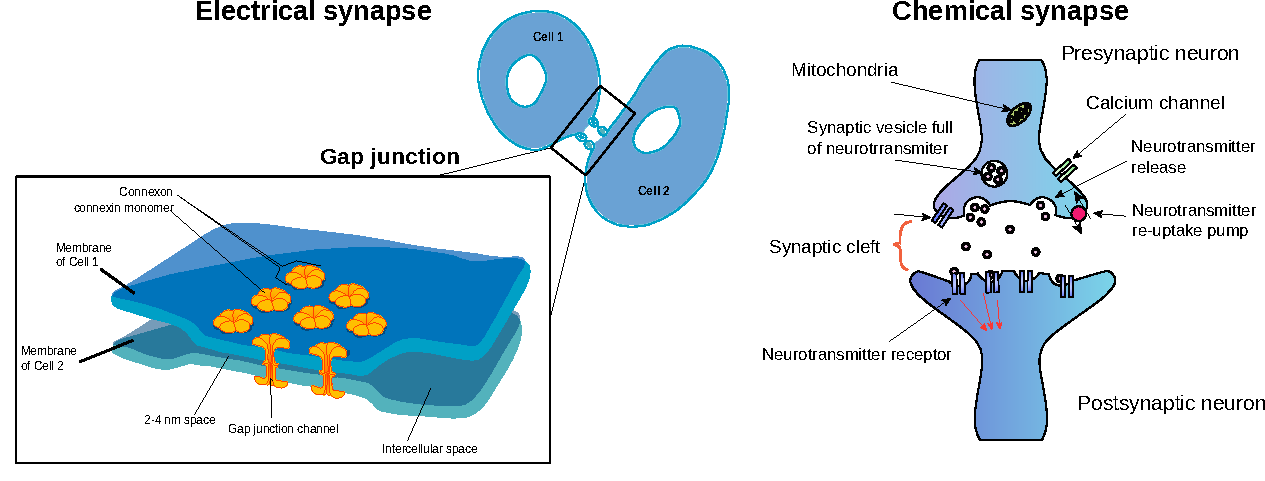
\includegraphics{img/intro/synapses.png}
    \caption{Representation of synapses types. Left. Example of electrical synapse structure. Right. Example of chemical synapse structure.}
    \label{fig:synapse-types}
\end{figure}

% As said there are many different ways to study neural dynamics, but a common descriptor for neural activity are action potentials. Action potentials are the 
Neural activity is often described by the potential alteration in the membrane caused by the flow of ionic channels and the conduction of nerve impulses by the axon. This variation of potential is called action potentials or spikes. We can see this as the minimal piece of information in the process of information reception, modification and transmission carried out by the neurons. A more concrete definition of spike could be "an abrupt and transient change of membrane voltage that propagates to other neurons via a long protrusion called an axon" \parencite{izhikevich_dynamical_2007}. Thus when no activity is transferred through the axon, the potential is called resting potential, main alterations to this potential are depolarization, when the potential is less negative than the resting potential, and hyperpolarization, when the potential is more negative than the resting potential. In figure \ref{fig:action potential} these potential phases are depicted. 

\begin{figure}[htb!]
    \centering
    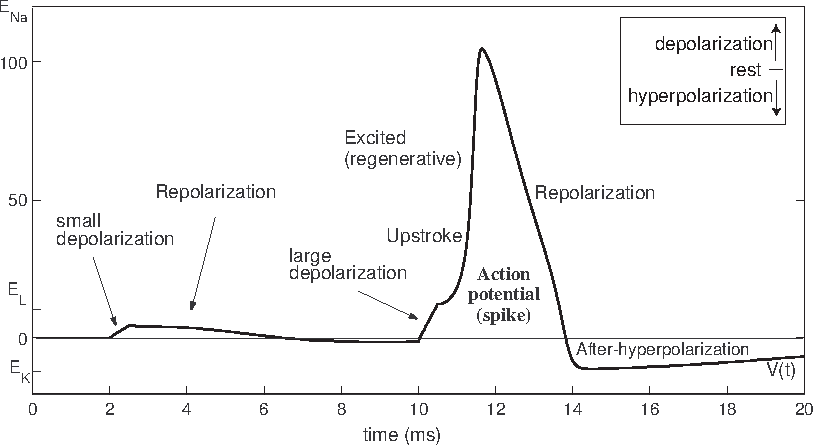
\includegraphics[width=\linewidth]{img/intro/dns_spike_phases.pdf}
    \caption{Representation of phases and terminology of an action potential. Adaptation of \textit{Figure 2.15: Action potential in the Hodgkin-Huxley model.} from book "Dynamical systems in neuroscience" \parencite{izhikevich_dynamical_2007}. }
    \label{fig:action potential}
\end{figure}
The membrane can be composed by different ionic channels, and its dynamics are conditioned by that combination and the possible synaptic connections. This changes in dynamics can be manifested in different ways, but the most notorious ones are the shape of the action potential and the type of activity that they show. %p61 The Neuron 
For example, in Figure \ref{fig:spike-types} there is an example of two distinct action potentials with visible differences in their shape. In Figure \ref{fig:spike_activity-types} there is an example of distinct neural activities from intracellular recordings. 
\begin{figure}[htb!]
    \centering
    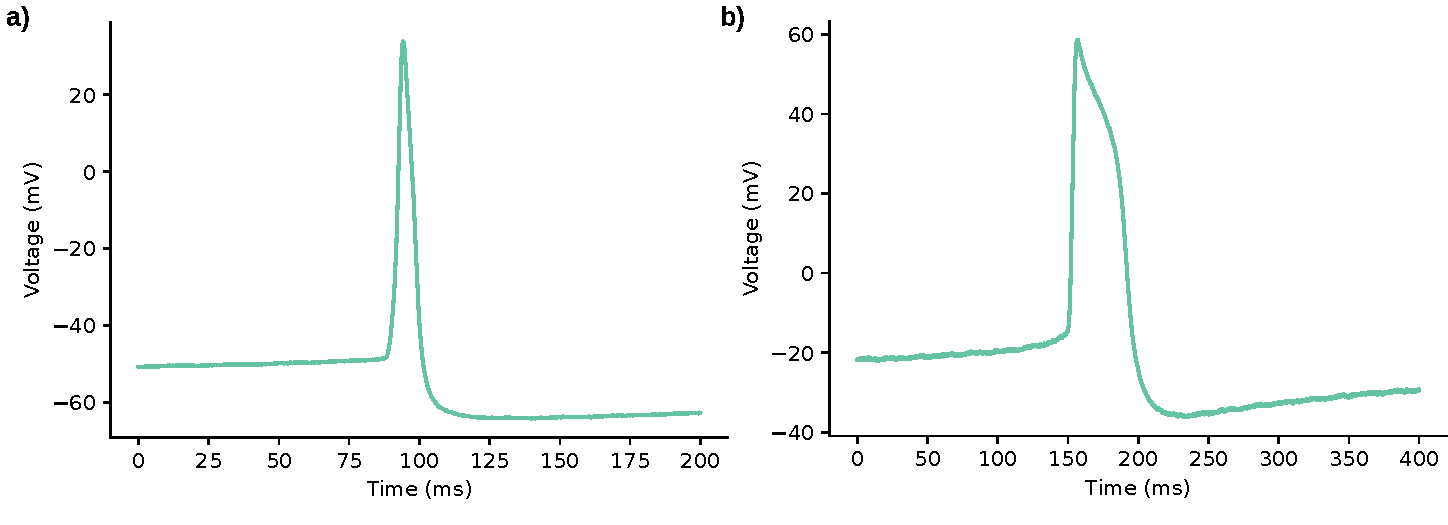
\includegraphics[width=\linewidth]{img/intro/spike-types.pdf}
    \caption{Examples of different spike shapes. Representation of two recordings from two different cells in \textit{Lymnaea stagnalis}. Left: symmetrical spike; right: shoulder shaped spike.}
    \label{fig:spike-types}
\end{figure}
\begin{figure}[htb!]
    \centering
    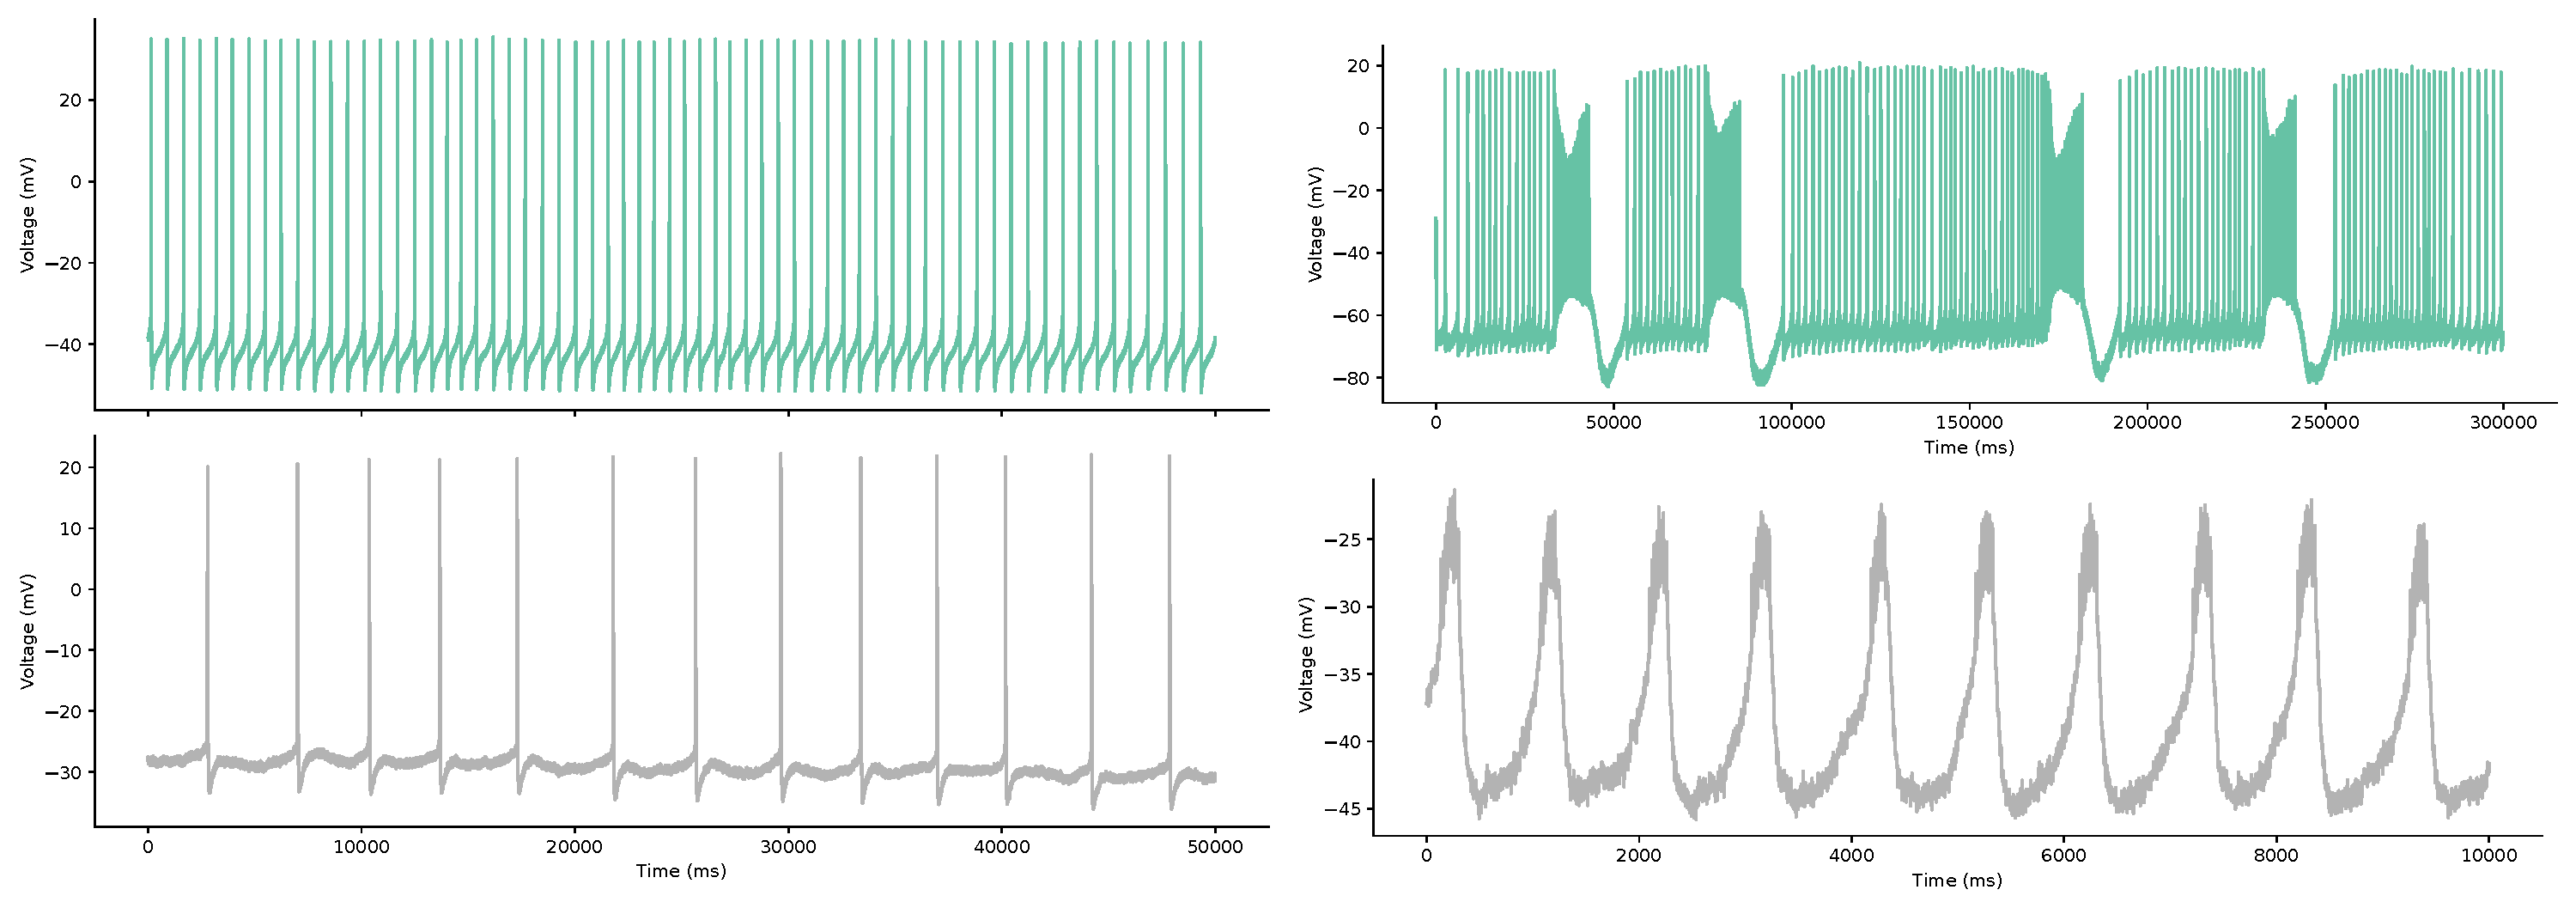
\includegraphics[width=\linewidth]{img/intro/spike_activity-types.pdf}
    \caption{Representation of different spiking activities. Left: two simultaneous intracellular recordings in \textit{Lymnaea stagnalis} showing tonic firing at two different frequencies. Right: Two examples of bursting activity, up from \textit{Lymnaea stagnalis} and bottom from \textit{Carcinus maenas}}
    \label{fig:spike_activity-types}
\end{figure}
If spikes are considered minimal pieces of information when coding the neural activity, the combination of these minimal information leads to new forms of information, also known as bursts. Although there is not a fixed description of a burst, and depending on the animal and system a burst might look different \parencite{russell_bursting_1978,palmu_detection_2010,lundqvist_gamma_2016}, there are some common features in bursts: combination of spikes (more than two), higher frequency, sustained depolarization, a hyperpolarization followed by a resting inter-burst period (IBI). Traditionally, neural code has been studied as information by the binarization of the activity i.e. an spike does or does not occur. Burst can also be part of this codification, either as a whole piece of information or as a complex box of data itself. "bursts are a family of firing patterns that trigger physiological mechanisms not engaged by the same number of spikes in relative isolation" \parencite{friedenberger_silences_2023}. Bursts can be originated either by internal activation, mostly by calcium channels or by the synaptic dynamics involving the corresponding cell (inhibition/excitation) (for an extended review see \parencite{friedenberger_silences_2023}). This is the case in Central Pattern Generators (CPGs) \parencite{Katz,steuer_central_2018} that will be discussed in detail bellow and in Chapter \ref{c-invariants-model}.

\section{The importance of sequential neural dynamics}
%the complex landscape of unanswered questions in the field of neuroscience, from a bottom-up approach. 
In the complex landscape of neuroscience, its study and conceptualization can be framed in three parts: hierarchy, if the study is bottom-up or top-down approach; ; and sequentiallity Among all the studies here present there is a common key: sequentially in neural dynamics. We can see most dynamics in the whole brain and behavior as a sequence of interactions, from molecules to motor movement. In this section we well see a review of the sequential nature of neurons and their information processing.

The structural differentiation in the 

% There are many important cognitive processes that rely in sequential processes such as perception, memory, decision making, attention and emotion. %Binding \parencite{Michel and coegin 2018, Ravinovich 2020, He 2018}.
% Sequentiallity involves complex pieces of dynamical activity, that when incapsulated as units, can be seen as a chain of events with sequential behaviour \parencite{Ravinovich,2023}.


% Sequential activvation for unsuppervised learning/activity.

%Principles of Brain Dynamics: Global State Interaction Book
%https://www.frontiersin.org/articles/10.3389/fnsys.2014.00219/full
%https://www.ncbi.nlm.nih.gov/pmc/articles/PMC8367843/


%Kiebel 2009
%"Dynamic sequences are generated on various time-scales"
%"Brain is a recognition system that uses an internal model of its environment"

%Kiebel 2008
%"Many aspects of brain function can be understood in terms of a hierarchy of temporal scales at which representations of the environment evolve"


Temporal processing can be defined as the decoding of a generated temporal code. A common example of temporal processing is usually the speech processing, where temporal structures play a key role \parencite{bibid}. Sequential patterns are present in the phrases structure, as a sequences of syllables and silences. In this line, an extended case of study is the birdsong, which has this similarity to human's speech, as they process sequences of syllables \parencite{fishbein_sound_2019}. Beyond speech, sequential processing is also present in the motor movement and coordination, from muscle activation to repetitive movements such as rhythmic tapping.

\begin{figure}[hbt!]
	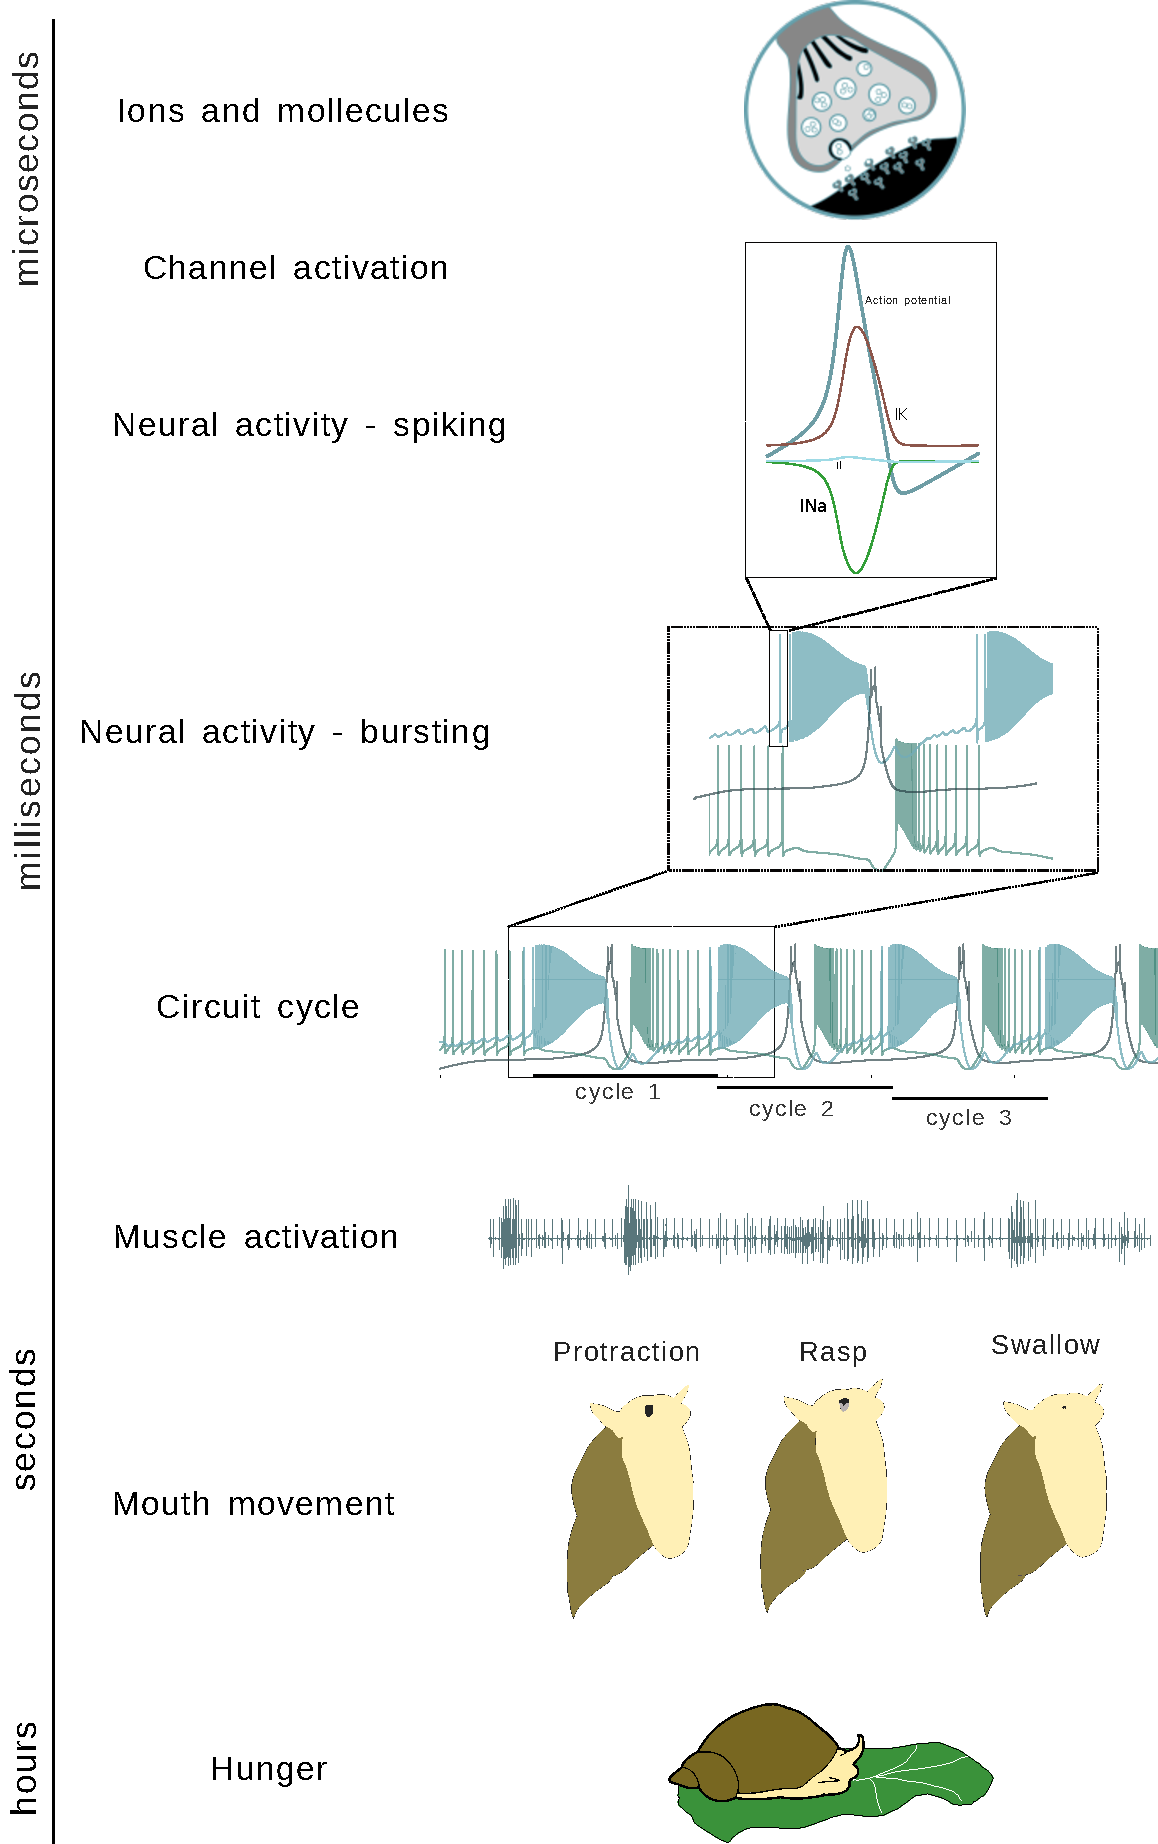
\includegraphics[width=0.9\textwidth]{img/intro/time scale/time-scale-feeding.pdf}
	\caption{Illustration of the sequential feeding process at different time scales.}
	\label{fig:time scale feeding}
\end{figure}

The sequential activity in brain goes from the scale of microsecond to days, as it is the example of circadian rhythms (see \cite{mauk_neural_2004}). We can also see this in the generation of coordinated motor activity as it is the case of the feeding of a snail. At the scale of microseconds, there is a flow of ions that generate a sequence of ionic channel activation, that in the scale of milliseconds, produce that produce action potentials that activate the corresponding muscles at the scale of seconds  and generate the necessary sequential movement to eat: open the mouth, rasp food and swallow. In figure \ref{fig:time scale feeding} there is an illustration of these scales.

However, it is not clear how exactly the brain processes time. In contrast to the theory of a central clock that manages time for every behavioral task, it is extended the theory of a distributed time processing \parencite{buonomano_temporal_1995,ivry_representation_1996}. For that to be processed, but maintaining effective responses, especially in movement, there is a need of circuits that manage the sequential movement.\todo{bibliografía} This is the case of Central Pattern Generators (CPGs), these are closed circuits of neurons that activate sequentially, in mutual inhibition and that generate coordinated motor activity in many systems, from insects to humans \parencite{bibid}. There are a few key aspects that makes this circuit an interesting case of study. First, the neurons in the closed-topology are able to maintain a rhythmic activity in an autonomous manner by mutual inhibition. Second, the activity is flexible enough to adapt to changes in the context, e.g., variations in the terrain while walking. Finally, it is present in many systems and in some of them there is a direct transcription between the neurons in the circuit and the motor movement they produce, e.g., the PD, LP and PY neurons in the stomatogastric CPG in the crab \textit{C. maenas} correspond to the pilo


\section{Computational Neuroscience}
Computational Neuroscience is a subfield of neuroscience that enhances the theoretical and computational techniques to address the study of nervous system functioning at multiple levels, from molecular level to complex networks or behavior. It is then by definition, a multi-disciplinary field. The basis of Computational Neuroscience lay on the understanding of brain dynamics from its electrical signals and the information they carry \parencite{schwiening_brief_2012,catterall_hodgkin-huxley_2012,dimitrov_information_2011,shannon_mathematical_1948}. Computational Neuroscience has extended its scope, leading to new paths o	f research including complex networks, graph theory, single cell analysis and machine learning techniques \parencite{cns2023}. Actually, in fields such as Artificial Intelligence there is a symbiotic relationship between fields, where both inspire and help each other grow \parencite{amunts_human_2019,wozniak_deep_2020,goncalves_training_2020}.

An important part of Computational Neuroscience is the description of living dynamics with theoretical models and the reproduction of their activity by the model simulation. The simulation of neural activity is a powerful tool to explore the neuronal dynamics, biophysical sources and possible mechanisms underlying the neural signaling, behavior, etc. Its strength relies on the reproducibility, extensive range of tunable parameters and the ability to modify (include/exclude) elements in the system or circuit. Like science is not about truth, but about knowledge, models do not aim to substitute living systems, but to lead us closer to the insight of neural dynamics. %#ToDo revisar

Models can be classified by their level of specification, i.e. what level of abstraction is decided in neural dynamics, the structure being modeled and the size of network and their ability to reproduce chaotic activity. In Figure \ref{fig:models-classification} there is a colored box illustrating this classification, with examples of models of large networks as \cite{potjans2014,bezaire2016}, of single cell but still detailed as in \cite{smith2013} and more abstract descriptions as in \cite{izhikevich}.


%Adapt models table from
%https://www.sciencedirect.com/science/article/pii/S0896627319304441 Figure 2A:
\begin{figure}[bth!]
	\centering
	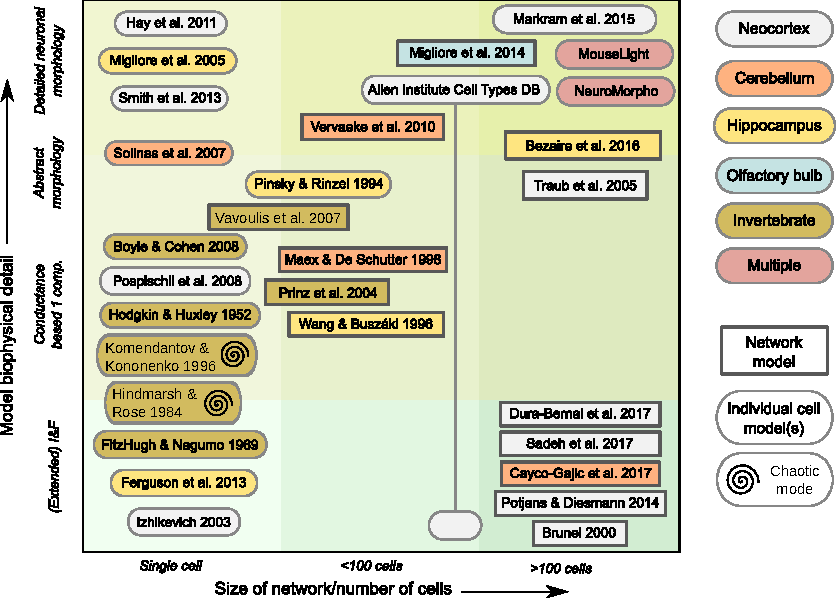
\includegraphics[width=\textwidth]{img/intro/models classification.pdf}
	\caption{Neural and network models classified by biophysical detail, structure modeled. Figure adapted from Figure 2 \cite{gleeson_open_2019}}
	\label{fig:models-classification}
\end{figure}
Although it was included in this classification, the capability of models to reproduce chaotic activity is often undervalued. Most studies use deterministic non-chaotic models, which are sufficient when exploring input/output responses, studying the role of different biophysical elements or supporting experimental results. However, living systems are chaotic and highly variable, and still able to produce sequential, constant and reproducible patterned activity. While this is a key aspect in neural dynamics, models usually exclude the variability from their description and include, when necessary Gaussian noise as external input to induce stochasticity. However, this is limited when exploring the role of variability in the sequences or in the information processing, inferring hypothesis from the model analysis.
\todo{mejorar justificación y añadir referencias de gaussian}
%#ToDo mejorar justificación y añadir referencias de gaussian.

\subsubsection{Conductance-based models}

In this thesis, all experimental recordings have been supported with simulations on conductance-based models. They can be defined as mathematical descriptions of the ionic channels dynamics, based on their electrical signal. The first description is usually assigned to \cite{hodgkin_quantitative_1952} model, that defined dynamical equations based on the electrical circuit of neurons in \textit{Aplysia}, see \ref{fig:electrical circuit}.

\begin{figure}[htb!]
	\centering
	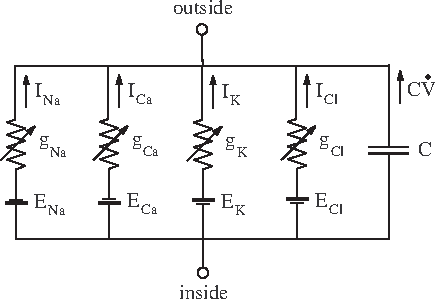
\includegraphics[width=0.7\textwidth]{./img/intro/dns_neuron_circuit.pdf}
	\caption{Electrical circuit representing membrane. Figure 2.3 from book "Dynamical systems in neuroscience" from \cite{izhikevich_dynamical_2007}.}
	\label{fig:electrical circuit}
\end{figure}

In this models, the simulation of neural electrical activity is based on the combination of different ionic channels, whose dynamics are also well defined with a description of activation gates which are also dynamically defined. The equations correspond to the following structure:

Dynamical Voltage time dependent:

\begin{equation}
 C_m \frac{dV}{dt} = I - \sum I_{x},
\end{equation}

where $I_{x}$ is the current description for each channel involved in the action potential generation, e.g. $I_K$, $I_{Na}$, $I_{Ca}$.

Each channel is also described as a differential equation, voltage-dependent composed by activation-gates dynamics:
\begin{equation}
I_x =  g_x \sum act_{vars}^n (V - E_x), 
\end{equation}

where $g_x$ is the corresponding conductance of the channel, $E_x$ is the reversal potential for that channel.
Activation gates usually have an exponential tendency, and are defined by activation and inactivation dynamics, also dependent on voltage and time. They follow the structure in equation \ref{eq:alpha-beta}

\begin{equation}
	\label{eq:alpha-beta}
	\frac{act}{dt} = \frac{act{\inf,i}-act_i}{\tau_{act,i}}
\end{equation}

where $\tau_{act,i}$ are the relaxation time constants which are usually voltage-dependent and modeled using sigmoid or Gaussian functions, as in equations \ref{eq:alpha-beta}. 


 An example of the equations corresponding to figure \ref{fig:electrical circuit} are:
\begin{equation}
		C V = I - g_K n^4 (V - E_K) - g_{Na} m^3h(V-E_{Na}) - g_L (V-E_L)
\end{equation}

\begin{multicols}{2}
	\begin{equation}
		n = \alpha_n (V)(1-n)-\beta_n(V)n
	\end{equation}
	\begin{equation}
		m = \alpha_m (V)(1-m)-\beta_m(V)m
	\end{equation}
	\begin{equation}
		h = \alpha_h (V)(1-h)-\beta_h(V)h
	\end{equation}


	\begin{equation}
	\alpha_n(V)=0.01\frac{10-V}	{\exp(\frac{10-V}{10})-1}
	\end{equation}
	\begin{equation}
	\beta_n(V)=0.0125\exp(\frac{-V}{80})
	\end{equation}


\vspace{-15pt}
	\begin{equation}
		\alpha_m(V)=0.1\frac{25-V}{\exp(\frac{25-V}{10})-1}
	\end{equation}
	\begin{equation}
		\beta_m(V)=4\exp(\frac{-V}{18})
	\end{equation}

\vspace{-15pt}
	\begin{equation}
	\alpha_h(V)=0.07\exp\frac{-V}{20}
	\end{equation}
	\begin{equation}
		\beta_h(V)=\frac{1}{\exp(\frac{30-V}{10})+1}
	\end{equation}
\end{multicols}


As in living systems, the combination of different channels lead to different activities, e.g. shoulder and no-shoulder type neurons showed in Figure \ref{fig:spike-types}, can be reproduced in models (see Fig. \ref{fig:spike-types model}). 

\begin{figure}[htb!]
	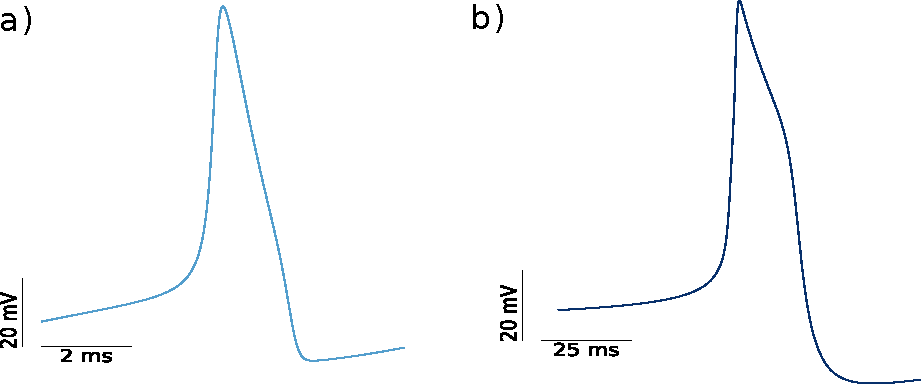
\includegraphics[width=\textwidth]{img/intro/spike-types model.pdf}
	\caption{text}
	\label{fig:spike-types model}
\end{figure}



\section{Study in invertebrates}
\label{c-intro-invertebrates}
Even before computational techniques were an option, the study of Neural dynamics and behavior was carried using many different model animals. Apart from the hegemonic rodents models, there have been invaluable findings using invertebrates as animal models, such as genetics and developmental biology in \textit{C. elegans} \parencite{brenner_genetics_1974}, \textit{Zebra fish} \parencite{streisinger_production_1981} and \textit{Drosophila} \parencite{nusslein-volhard_mutations_1980}; neural dynamics in \textit{Aplysia} \parencite{HODGKIN1952,wachtel_direct_1967}, motor activity in \textit{Carcinus maenas} \parencite{eisen_mechanisms_1982} or \textit{Lymnaea stagnalis} \parencite{Benjamin1979b}, the main animal model in this thesis. Those are only examples of fields, these animal models have been used for a wide variety of fields including behavioral studies, ecotoxicology, evolution, human disease modelling... \parencite{romanova_animal_2018} 

Despite the differences between invertebrates, mammals and concretely human brain, there are many characteristics of animals' systems that can be extrapolated to humans. In fact, there are differences even in mammal species \parencite{preuss_taking_2000}, so by exploring more animal species there can be set a better ground truth for the aspects that shape the neuronal and behavioral dynamics. 

 % https://karger.com/bbe/article-abstract/55/6/287/46613/Taking-the-Measure-of-Diversity-Comparative?redirectedFrom=fulltext  
 %First, by examining a wider range of species than are currently employed, and by using modern techniques of phyletic analysis, neuroscientists can more rigorously identify those features of cortical organization that are, in fact, widely shared among mammals or among particular mammalian subgroups. Second, by taking account of variations, neuroscientists can abstract more reliable and general principles of structure-function relationships in the nervous system. Finally, freed from the doctrine of basic uniformity, neuroscientists can pursue the study of human cortical specializations, and so advance our understanding of what distinguishes humans as a biological species.

Among the advantages in using invertebrates there are the easy access to the nervous system, the ease of breeding and reproduction, the simplicity of their biological features, making a full description possible, i.e. the genomic description of \textit{C. elegans} or the nervous system in \textit{Lymnaea stagnalis}. Also some selected species were a main field of study in the last decades, so there is plenty of literature for each one even in different fields. Furthermore, despite the simplicity of these systems, their nervous system is still capable of generating robust sequential neural activity, preset behavior and even learning processes. 

Findings in invertebrates are sometimes overlooked, arguing that features in invertebrates cannot be extrapolated to humans. Thus, there are often used mammals by their biological similarity. However, models in invertebrates have proven their utility not only in basic science. We can find examples of this in human diseases, memory, motor activity and neuromodulation. Particularly, in the study of neural processes, the ease of accessibility and finite number of large neurons in the system, have made invertebrates an interesting case of study. In Figure \ref{fig:invertebrates timeline} there is a timeline containing crucial discoveries in Neuroscience, some of them Nobel Prize winners in the last century, as well as current relevant discoveries in the field. 
% https://docs.google.com/spreadsheets/d/16rOG5LSuFMQGHAakeYqcdG26NIZnY4NWtr6TZku_UKs/edit#gid=0

Apart from the possible advances in science, invertebrates models can also bridge the gap between resources and science, allowing low-income labs and countries to do science. This animal models are usually cheaper to obtain, maintain and there is usually a possibility of breeding own colonies. This makes their use extendable and breaks some economical barriers in science, where high-income countries usually centralize the science production with strong conventions \parencite{castillo_spineless_2017,stephan_how_2015}. 

\textit{What can computational neuroscience provide to experimental approaches}



\subsubsection{\textit{Lymnaea stagnalis}, the great pond snail}
Besides the potential of research in invertebrates in general, here we explore neural system in the great pond snail, \textit{Lymanea stagnalis}. This mollusk has been an important case of study since the late XX century, when it was used extensively to study neurobiological processes and nervous system functioning \parencite{Benjamin1979a}. %#TODO: repaso de Benjamin

\begin{wrapfigure}{l}{0.3\textwidth}
	\centering
	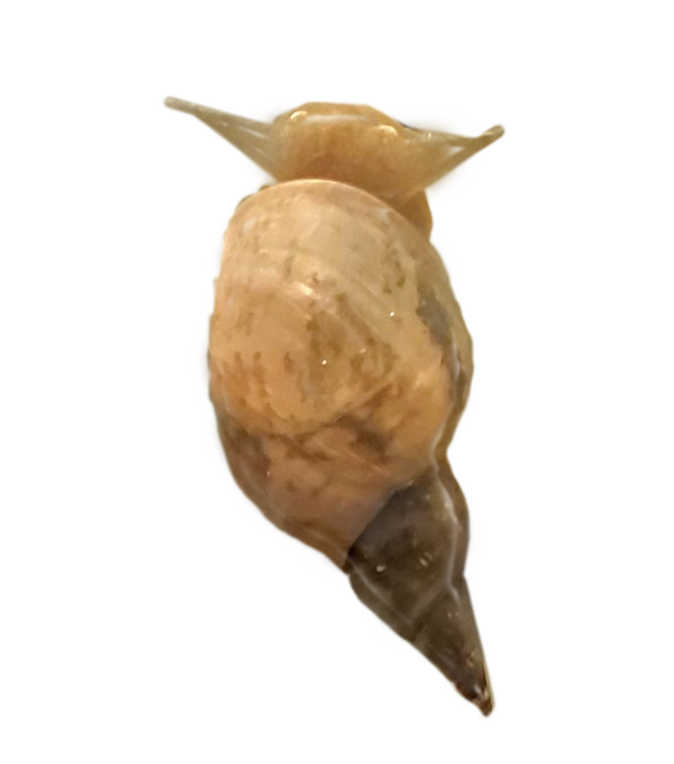
\includegraphics[width=0.7\linewidth]{img/intro/lymnaea.png} 
	\caption{\textit{Lymnaea Stagnalis}}
	\label{fig:snail}
\end{wrapfigure}  From that point on it has been key in other fields as host-parasite or genome editing. This last field is thanks to the short and well studied life-cycle in \textit{L. stagnalis} (see Figure \ref{fig:lymnaea_life_cycle}), as well as the easiness to lab-bread them, without losing its main characteristics through generations \parencite{noland_observations_1946}. 


\begin{figure}[htb!]
	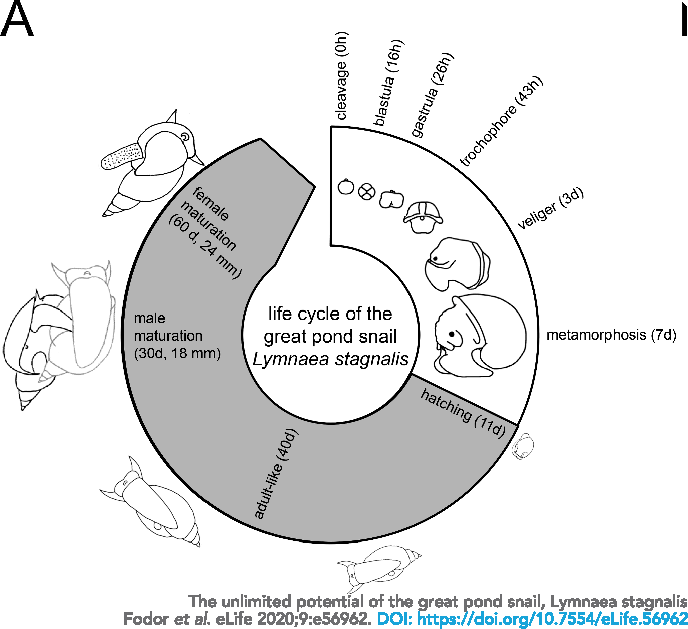
\includegraphics[width=\textwidth]{img/intro/lymnaea_life_cycle.pdf}
	\caption{text}
	\label{fig:lymnaea_life_cycle}
\end{figure}




\section{Neuromodulation and its need for clinical applications}